\documentclass[aps,pra,twocolumn]{revtex4-2}
\usepackage{amsmath,amsfonts,amsthm,bbm}
\usepackage[dvipsnames]{xcolor}
\usepackage{graphicx}
\usepackage{multirow,mhchem,chemformula}
\usepackage[colorlinks=true,breaklinks=true,linkcolor=red,citecolor=magenta,urlcolor=magenta]{hyperref}

\usepackage{tikz}
\usetikzlibrary{quantikz}

\newcommand{\crt}[1]{\hat{c}_{#1}^\dagger}
\newcommand{\dst}[1]{\hat{c}_{#1}^{\phantom{\dagger}}}
\newcommand{\vett}[1]{{\bf{#1}}}
\newcommand{\bgreek}[1]{{\boldsymbol{#1}}}

\begin{document}

\title{Accuracy assessment of quantum computing algorithms for chemistry: \\
a numerical study of variational Ans\"{a}tze across a database of problems}

\author{IBM authors}
\affiliation{IBM Quantum, IBM Research Almaden, 650 Harry Road, San Jose, CA 95120, USA}
\author{Virginia Tech authors}
\affiliation{Department of Chemistry, Virginia Tech, 480 Davidson Hall, Blacksburg, VA 24061, USA}

\begin{abstract}
\end{abstract}

\maketitle

\section{Introduction}

Recent years have witnessed remarkable research in the simulation of many-body quantum systems  by quantum computing algorithms.
A prominent application targeted by quantum algorithms is the electronic structure (ES) problem, 
namely solving for the ground or low-lying eigenstates of the electronic Schr\"{o}dinger equation for atoms, molecules, and materials.
Research in this direction has delivered promising results in the calculation of potential energy curves, 
ground- and excited-state energies and correlation functions for various instances of the ES problem.

Notwithstanding these rapid developments, the behavior of quantum computing algorithms for the ES problem remains to be understood and established,
and such a situation is due to several factors. For example: 
different research groups demonstrate existing or novel algorithms on different instances of the ES problem, which makes comparative algorithm analysis difficult;
the design and implementation of novel quantum computing algorithms is often coupled to their demonstration on contemporary quantum hardware, which restricts the domain of potential applications to very small numbers of electrons and orbitals;
the limitations of classical simulators have similarly resulted in most simulations reported to date being restricted to very small instances of the ES problem, so that the observed algorithmic behavior is not guaranteed to generalize to larger or more complex instances;
even when quantum algorithms have known limitations, their numeric assessment is often limited by the immaturity of contemporary quantum computational platforms, which makes difficult to gauge the severity of such limitations.

Overcoming these limiting factors can contribute to the understanding of the nature, performance and limitations of quantum algorithms for the ES problem, and bring progress in their design and assessment.
Useful steps towards this goal are:
to establish a database of problems that different researchers can use to test quantum algorithms;
to propose a set of metrics to quantify algorithmic performance, and support an objective comparison of algorithmic behavior;
to establish a database of results that different researchers can consult to compare and contrast quantum algorithms.

The proposed problems should be sufficiently simple, to be demonstrated on contemporary quantum computing platforms, and non-trivial, to ensure meaningful assessments of algorithmic behavior.
Moreover, the assessment of algorithmic behavior should decouple classical simulators of quantum devices and actual quantum devices,
so that theoreticians can explore the properties of a methodology assuming an ideal quantum device, and experimentalists can independently test a set of well-defined quantum circuits motivated by the solution of instances of the ES problem.
 
In this work, we present a set of instances of the ES problem, and perform an assessment of Ans\"{a}tze used in variational ground-state quantum simulations,
using classical simulators of quantum hardware.
In the assessment of quantum algorithms, we will use the difference between the computed and exact ground-state energy as an indicator of algorithmic quality,
along with the expectation values of quantities signaling the breaking of Hamiltonian symmetries, a conceptually important but often overlooked aspect of variational quantum simulations.
We will use a variety of indicators of algorithmic cost, related to the optimization of variational parameters (number of variational parameters, cost of energy evaluation)
and to the quantum circuits leading to the calculation of energies and properties (number of qubits, gates and measurements, circuit depth).

As illustrative applications, we employ the database presented here to test a new variational Ansatz termed {\em{cascade}} against existing methods,
to compare open- and closed-shell implementations of the unitary coupled-cluster with singles and doubles \cite{scuseria1987closed,szalay1997spin}, 
and to compare two different strategies to encode fermionic degrees of freedom to qubits.

The remainder of this work is organized as follows: 
in Section \ref{sec:methods} we describe the proposed database, and the algorithms tested in the present work;
in Section \ref{sec:results} we present the results of this study;
conclusions and perspective prosecutions of this work are describe in Section \ref{sec:conclusions},
and an appendix contains additional computational details.

\section{Methods}
\label{sec:methods}

In this section, we present the problems constituting the database studied in this work,
and the metrics used to establish algorithm performance and computational cost.

\subsection{Target problems}

In this work, we focus on a set of four molecular species, namely BH, HF, BeH$_2$, and H$_2$O.
The BH, HF, BeH and OH bondlengths $R$ vary between 0.5 and 3.5, 4.5, 4.5, and 3.3 Angstrom respectively.
These molecular species, proposed in previous works, allow to test quantum algorithms along the breaking of one (BH and HF) or two (BeH$_2$, and H$_2$O) covalent bonds,
and in presence of dominant dynamic (small $R$) or static (large $R$) electronic correlation.

For each species, a restricted closed-shell Hartree-Fock calculation is performed, as specified in Appendix \ref{sec:classical}.
The core 1s orbital is frozen and the Born-Oppenheimer Hamiltonian
\begin{equation}
\label{eq:hamiltonian}
\hat{H} = E_0 + \sum_{\substack{p r \\ \sigma}} h_{p r} \crt{p \sigma} \dst{r \sigma} + \sum_{\substack{p r q s \\ \sigma\tau}} \frac{(pr|qs)}{2} \crt{p \sigma} \crt{q \tau} \dst{s\tau}  \dst{r \sigma}
\end{equation}
is computed, along with the number, spin-$z$, and total spin operators
\begin{equation}
\label{eq:auxiliary}
\begin{split}
\hat{N} &= N_f + \sum_{p \sigma} \crt{p \sigma} \dst{p \sigma} \quad, \\
\hat{S}_z &= \sum_{p \sigma} (-1)^\sigma \crt{p \sigma} \dst{p \sigma} \quad, \\
\hat{S}^2 &= \sum_{pq} \crt{p\downarrow} \dst{p\uparrow} \crt{q\uparrow} \dst{q\downarrow}   + \hat{S}_z (\hat{S}_z-1) \quad,
\end{split}
\end{equation}
where $N_f = 2$ is the number of frozen electrons. 
In this study we focused on a minimal STO-6G basis, to ensure a number of orbitals and qubits within the reach of contemporary classical simulators of quantum circuits.

\subsection{Qubit encodings}

In the majority of quantum algorithms for contemporary devices, the Hamiltonian Eq.~\eqref{eq:hamiltonian} and the auxiliary operators Eq.~\eqref{eq:auxiliary} are mapped onto qubit operators,
and more specifically onto linear combinations 
\begin{equation}
\label{eq:qubit}
\hat{H} = \sum_{i=0}^{n_p-1} c_i \, \sigma_{\vett{v}_i \, \vett{w}_i} 
\quad,\quad
\sigma_{\vett{v} \, \vett{w}} = \bigotimes_{k=0}^{n_q-1} \sigma_{v_k w_k} 
\quad,
\end{equation}
of Pauli operators acting on a certain number $n_q$ of qubits. In Equation~\eqref{eq:qubit} $\sigma_{00,01,10,11} = \mathbbm{1},X,Z,Y$ is a single-qubit Pauli operator, 
$c_i$ a real-valued coefficient, and the summation ranges over $n_p$ terms.

In this study, we employ both second-quantization and first-quantization encodings.
The former establish a one-to-one mapping between the Fock space of electrons in $M$ spatial orbitals and the Hilbert space of $n_q = 2M$ qubits,
and the latter between the Hilbert space spanned by a set of $K$ space- and spin-adapted configuration state functions (CSFs) and the Hilbert space of $n_q = \lceil \log_2 K \rceil$ qubits.

First-quantization encodings ensure access to automatically symmetry-adapted many-electron wavefunctions, and require less qubits than their second-quantization counterparts.
However, they are less straightforward to implement, and lead to a representation of the Hamiltonian where $n_p$ scales exponentially with $n_q$.
Additional technical details are provided in Appendix \ref{sec:first}.

Second-quantization encodings give rise to a compact representation of the Hamiltonian and of auxiliary operators as linear combinations of a polynomial number of Pauli operators,
but allow the possibility that Hamiltonian symmetries are broken, for multiple reasons discussed in Section \ref{sec:metrics}.
To alleviate the latter issue, we combine the parity mapping with the two-qubit and tapering techniques. The former removes two qubits to ensure conservation of the parity operators
$(-1)^{\hat{N}_\uparrow}$ and $(-1)^{\hat{N}_\downarrow}$, and the latter identifies a subgroup of the symmetry group isomorphic to $\mathbb{Z}_2^{\times k}$ and removes $k$ qubits
to ensure the simulated wavefunctions lie in a target irreducible representation of the identified subgroup. The species studied here have symmetry groups 
($C_{\infty v}$ for BH and HF, $D_{\infty h}$ for BeH$_2$ and $C_{2v}$ for H$_2$O) isomorphic to $\mathbb{Z}_2 \times \mathbb{Z}_2$, so that the combined use of two-qubit reduction
and tapering leads to $n_q = 2M-4$ qubits.

\subsection{Target variational Ans\"{a}tze}

In this study, we elected to explore the behavior of the variational quantum eigensolver (VQE) algorithm, due to its widespread adoption in the community.
This method defines a set of Ansatz states approximating the ground state of a target Hamiltonian, of the form 
\begin{equation}
| \Psi( \bgreek{\theta} ) \rangle = \hat{U}( \bgreek{\theta} ) | 0 \rangle^{\otimes n_q}
\quad,
\end{equation}
where $\bgreek{\theta} \in [0,2\pi)^{n_\theta}$ is an array of angles that define a parametrized quantum circuit $\hat{U}( \bgreek{\theta} )$, 
applied to a register of $n_q$ qubits prepared in the standard initial state $| 0 \rangle^{\otimes n_q}$.
The best approximation to the ground state in the set of Ansatz states is found by minimizing the energy 
\begin{equation}
E_{\mathrm{VQE}}( \bgreek{\theta} ) = \langle \Psi( \bgreek{\theta} ) | \hat{H} | \Psi( \bgreek{\theta} ) \rangle
\end{equation}
as a function of the parameters $\bgreek{\theta} $ using a classical optimization algorithm. 
Once the parameters are optimized, auxiliary observables can be measured, yielding results
\begin{equation}
X_{\mathrm{VQE}}( \bgreek{\theta} ) = \langle \Psi( \bgreek{\theta} ) | \hat{X} | \Psi( \bgreek{\theta} ) \rangle
\quad.
\end{equation}
This algorithmic workflow, termed variational quantum eigensolver (VQE) in the quantum simulation literature, 
is a heuristic technique for ground-state approximation. 
Its accuracy and computational cost, as discussed in Section \ref{sec:metrics}, are determined by the details of the circuit $\hat{U}( \bgreek{\theta} )$. 
In the remainder of this Section, we will present the Ans\"{a}tze assessed in the present work.

\subsubsection{Unitary coupled cluster with singles and doubles}

The quantum unitary coupled cluster (q-UCC) method is based on the exponential Ansatz, i.e., the exact wave function is written as
\begin{equation}
| \Psi_{\mathrm{gs}} \rangle = e^{ \hat{T} - \hat{T}^\dagger } | \Phi_0 \rangle
\end{equation}
where $\Phi_0$ is an independent particle function (here, the Hartree-Fock state) and $\hat{T}$ is a cluster operator which, 
at the singles and doubles level (q-UCCSD) is truncated to
\begin{equation}
\label{eq:unrestricted_quccsd}
\begin{split}
\hat{T} &= \hat{T}_1 + \hat{T}_2 \quad, \\
\hat{T}_1 &= \sum_{\substack{ai \\ \sigma}} t^{a \sigma}_{i \sigma} \crt{a \sigma} \dst{i \sigma} \quad,\\
\hat{T}_2 &= \sum_{\substack{abij \\ \sigma\tau}} t^{a\sigma \; b\tau}_{i\sigma \; j\tau} \crt{a \sigma} \crt{b \tau} \dst{j \tau} \dst{i \sigma} \quad,\\
\end{split}
\end{equation}
where $t^{a}_i$ and $t^{ab}_{ij}$ are a set of unknown cluster coefficients. We have adopted the convention that $i,j,k,l$ and $a,b,c,d$
refer to occupied and unoccupied orbitals in the reference configuration $\Phi_0$ respectively.
It should be noted that the form Eq.~\eqref{eq:unrestricted_quccsd}, presented in previous literature along with the corresponding quantum circuit,
corresponds to an unrestricted Ansatz, which is not guaranteed to yield an eigenfunction of total spin.

If a closed shell spin-adapted formalism is used, then, following Paldus and Scuseria et al, we need to have
\begin{equation}
t^{a \alpha}_{i \alpha} = t^{a \beta}_{i \beta} = t^a_i \quad,
\end{equation}
since the two other possible spin combinations are vanishing. 
Only 6 of the 16 possible spin combinations for the two-electron amplitudes are non-zero, namely
\begin{equation}
\begin{split}
t^{a \alpha \; b \alpha}_{i \alpha \; j \alpha} = t^{a \beta \; b \beta}_{i \beta\; j\beta} = \hat{t}^{ab}_{ij} \\
t^{a \alpha \; b \beta}_{i \alpha \; j \beta} = t^{a \beta \; b \alpha}_{i \beta\; j\alpha} = \tilde{t}^{ab}_{ij} \\
t^{a \beta \; b \alpha}_{i \alpha \; j \beta} = t^{a \alpha \; b \beta}_{i \beta\; j\alpha} = \overline{t}^{ab}_{ij} \\
\end{split}
\end{equation}
Using the relations
\begin{equation}
\hat{t}^{ab}_{ij} = \tilde{t}^{ab}_{ij} + \overline{t}^{ab}_{ij}
\quad,\quad
\tilde{t}^{ab}_{ij} = - \overline{t}^{ab}_{ji} = - \overline{t}^{ab}_{ij} = \tilde{t}^{ba}_{ji}
\quad,
\end{equation}
one is left with only one set of independent two-electron amplitudes $\tilde{t}^{ab}_{ij}$ and $(ai) \leq (bj)$. In addition to reducing the 
number of variational parameters, the use of a closed shell spin-adapted formalism ensures that the cluster operator commutes with 
the total spin operator, $[ \hat{T} , \hat{S}^2 ] = 0$.
Its exponential, however, cannot be implemented exactly at polynomial cost on a quantum computer. 
Instead, as discussed in Appendix \ref{sec:cc_trotter}, a Trotter approximation is required, which in turn leads to spin symmetry breaking.

\subsubsection{Hardware-efficient $R_y$}

\subsubsection{Cascade}

% Ry Ansatz
% role of initial BS?
% q-UCCSD unrestricted/restricted
% cascade

\subsection{Metrics of algorithm performance}
\label{sec:metrics}

A natural metric to assess the accuracy of a variational simulation is the difference between the computed and exact ground-state energy, 
\begin{equation}
\Delta E = E_{\mathrm{VQE}}(\bgreek{\theta}) - E_{\mathrm{FCI}}
\quad .
\end{equation}
The ES Hamiltonian has several symmetries, i.e. operators $\hat{S}$ such that $[\hat{H},\hat{S}]=0$. 
In presence of Hamiltonian symmetries, the search for Hamiltonian eigenfunctions has to be restricted to eigenspaces of Hamiltonian symmetries with known eigenvalues.
Relevant Hamiltonian symmetries are the auxiliary operators Eq.~\eqref{eq:auxiliary}
and, for the molecules studied in the present work, the ground state lies in the eigenspaces of $\hat{S}_z$ and $\hat{S}^2$ with eigenvalue zero,
and of $\hat{N}$ with eigenvalues $6$ for BH and BeH$_2$ and 10 for HF and H$_2$O.

In general, a variational quantum simulation does not preserve Hamiltonian symmetries. To assess whether a variational simulation
leads to symmetry breaking, and to quantify its extent, we compute the deviations
\begin{equation}
\begin{split}
\Delta N &= N_{\mathrm{VQE}}(\bgreek{\theta}) - N_{\mathrm{FCI}} \quad, \\
\Delta S_z &= S_{z,\mathrm{VQE}}(\bgreek{\theta}) - S_{z,\mathrm{FCI}} \quad, \\
\Delta S^2 &= S^2_{\mathrm{VQE}}(\bgreek{\theta}) - S^2_{\mathrm{FCI}} \quad, \\
\end{split}
\end{equation}
between the computed and exact ground-state particle number, spin-$z$, and total spin.

In addition to the accuracy of a variational simulation, it is also important to quantify its computational cost. To this end we employ a tuple of values,
namely: 
the number of qubits $n_q$,  
the number of gates $n_g$ and the depth $d$ of the variational circuit, 
the number of Pauli operators in the Hamiltonian $n_p$, 
and the number of variational parameters $n_{\bgreek{\theta}}$.

\section{Results}
\label{sec:results}

\begin{figure*}[t!]
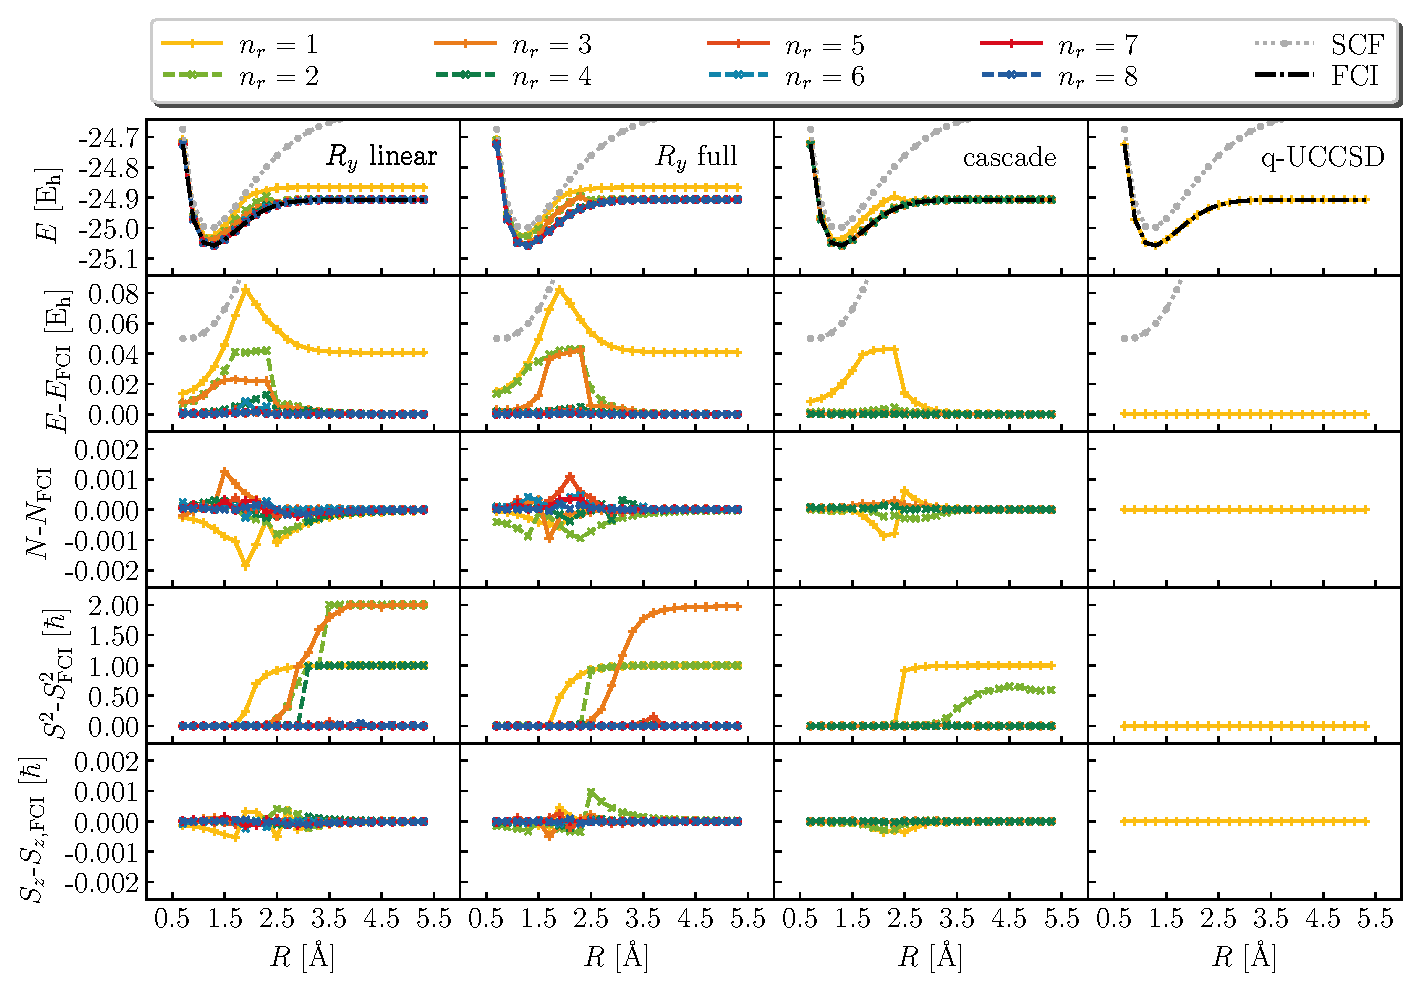
\includegraphics[width=0.8\textwidth]{../figures/second_quantization_bh/second_quantization_bh.eps}
\caption{Total energy, deviation between computed and exact total energy, electron number, total spin, and spin-$z$ (top to bottom) 
using the R$_y$ (with linear and full connectivity), cascade, and q-UCCSD Ans\"{a}tze (left to right), for the BH molecule at STO-6G level.}
\label{figure:second_bh}
\end{figure*}

\begin{figure*}[t!]
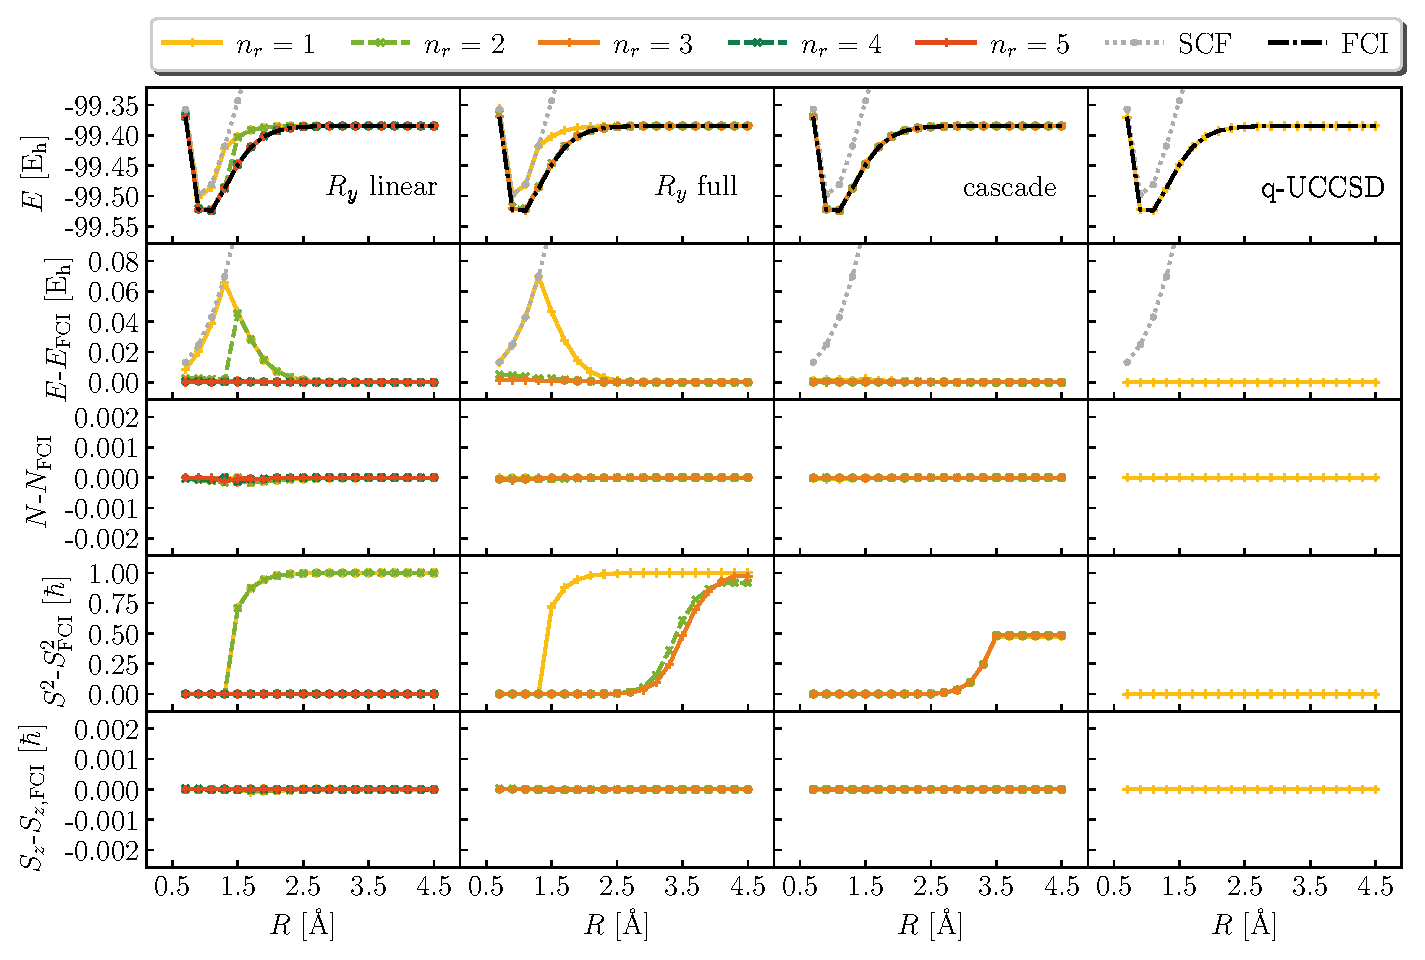
\includegraphics[width=0.8\textwidth]{../figures/second_quantization_hf/second_quantization_hf.eps}
\caption{Total energy, deviation between computed and exact total energy, electron number, total spin, and spin-$z$ (top to bottom) 
using the R$_y$ (with linear and full connectivity), cascade, and q-UCCSD Ans\"{a}tze (left to right), for the HF molecule at STO-6G level.}
\label{figure:second_hf}
\end{figure*}

\begin{figure*}[t!]
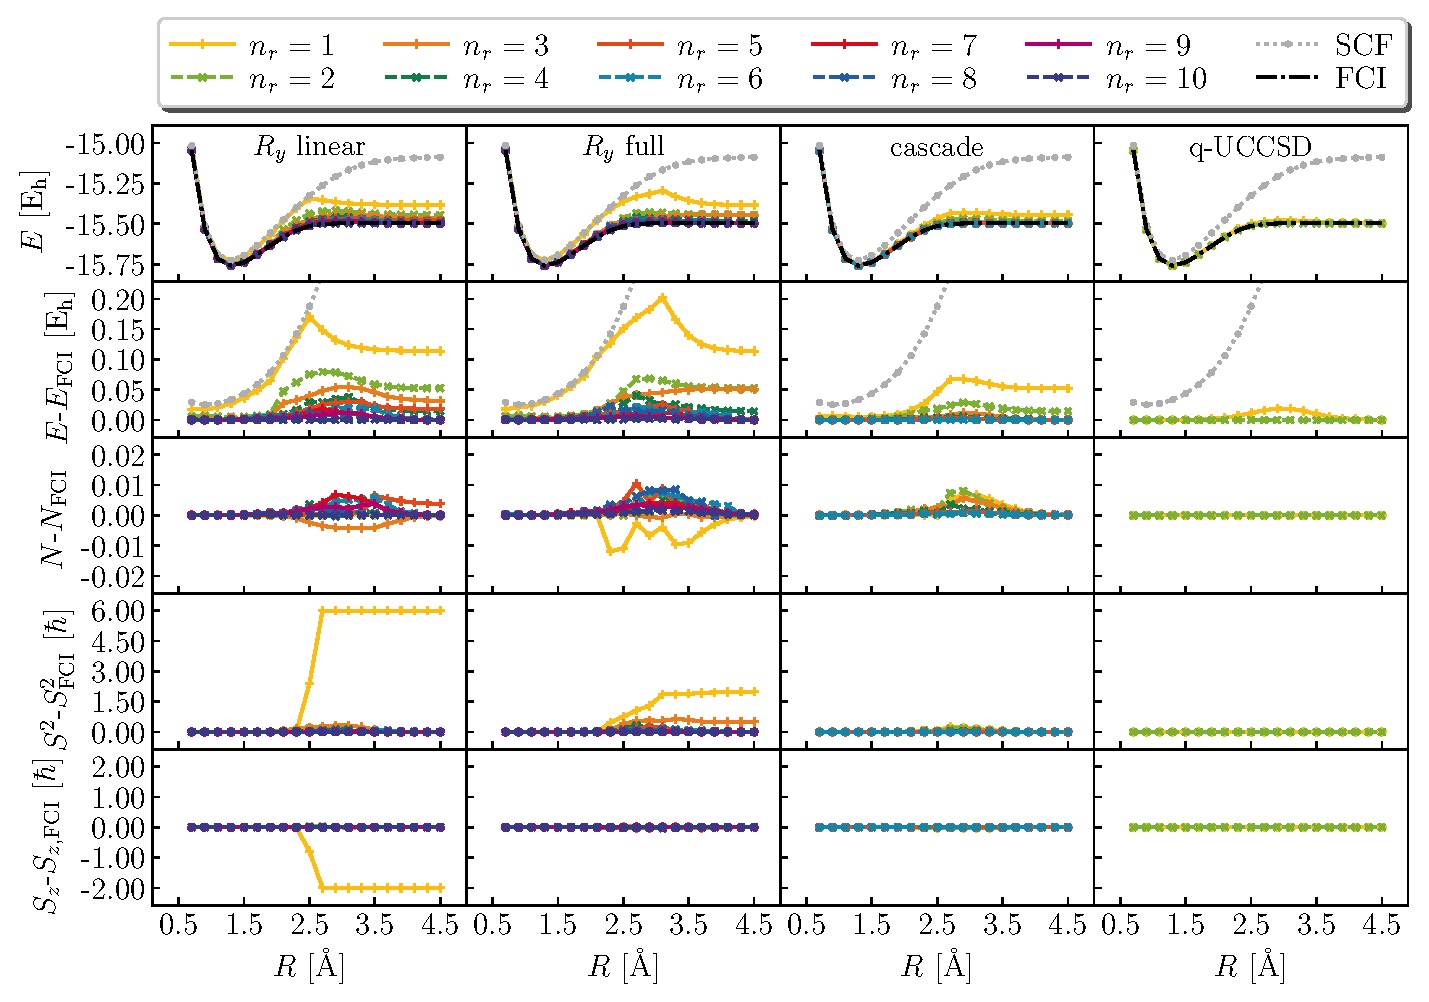
\includegraphics[width=0.8\textwidth]{../figures/second_quantization_beh2/second_quantization_beh2.eps}
\caption{Total energy, deviation between computed and exact total energy, electron number, total spin, and spin-$z$ (top to bottom) 
using the R$_y$ (with linear and full connectivity), cascade, and q-UCCSD Ans\"{a}tze (left to right), for the BeH$_2$ molecule at STO-6G level.}
\label{figure:second_beh2}
\end{figure*}

\begin{figure*}[t!]
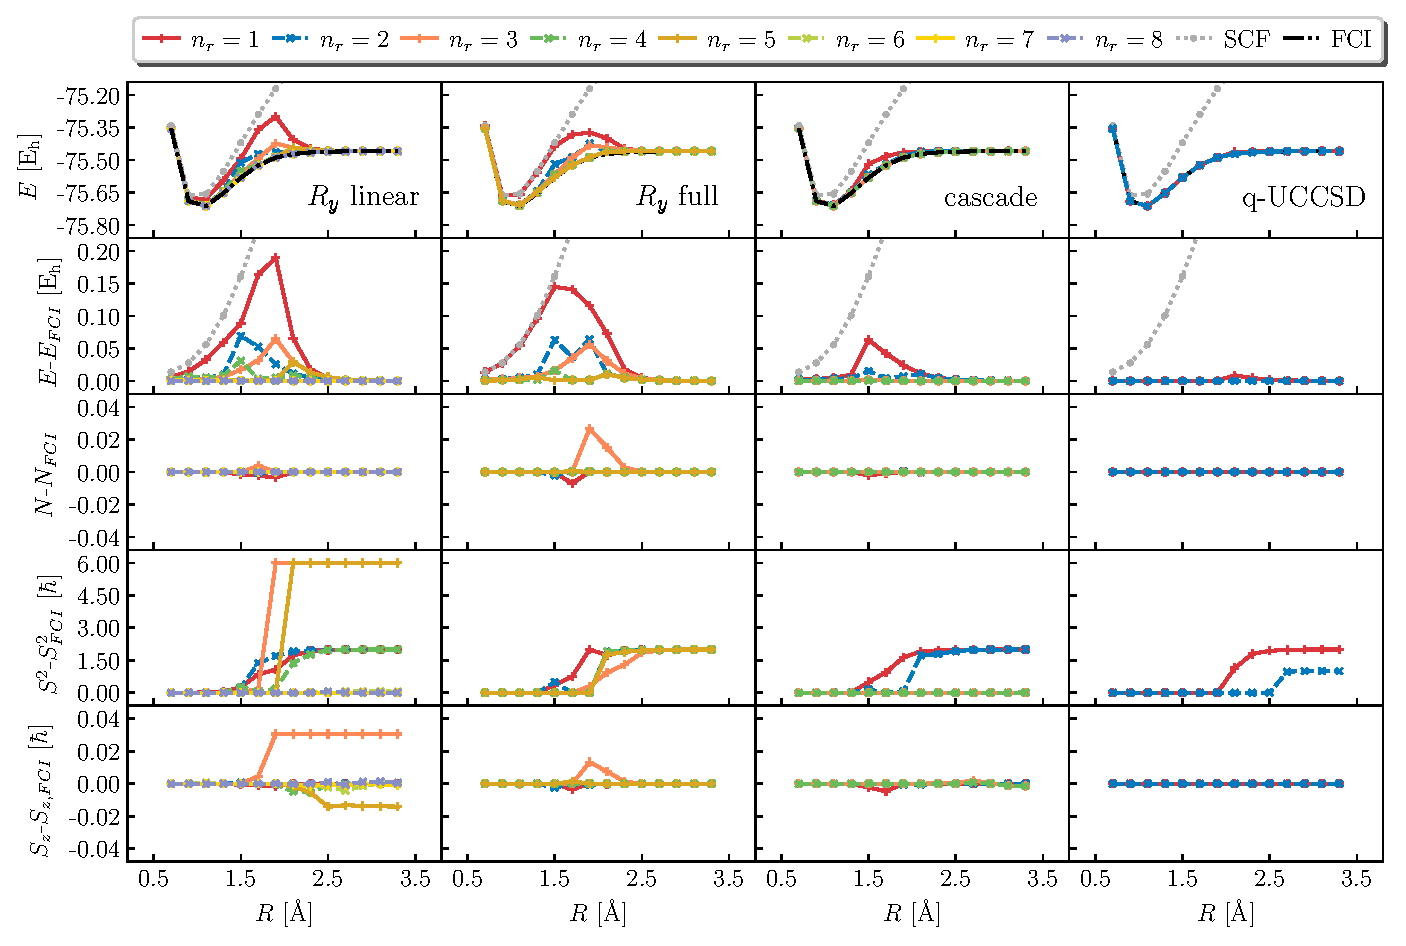
\includegraphics[width=0.8\textwidth]{../figures/second_quantization_h2o/second_quantization_h2o.eps}
\caption{Total energy, deviation between computed and exact total energy, electron number, total spin, and spin-$z$ (top to bottom) 
using the R$_y$ (with linear and full connectivity), cascade, and q-UCCSD Ans\"{a}tze (left to right), for the H$_2$O molecule at STO-6G level.}
\label{figure:second_h2o}
\end{figure*} 

\begin{figure*}[t!]
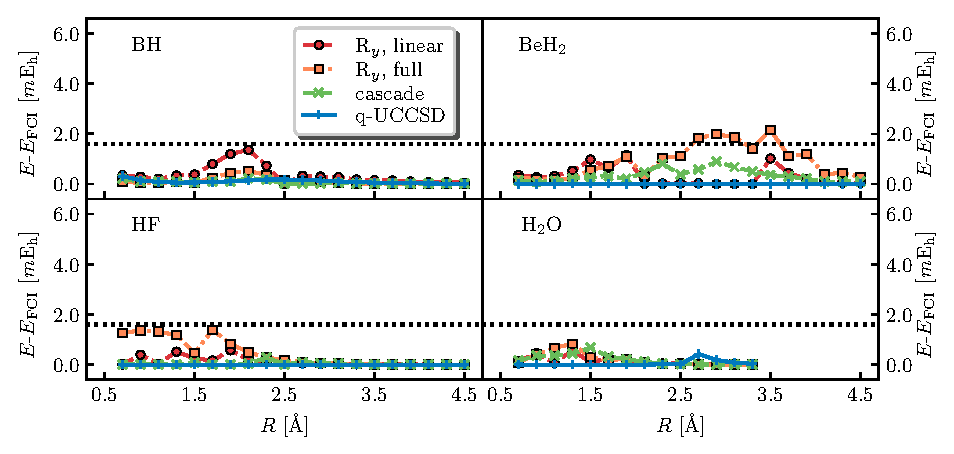
\includegraphics[width=0.7\textwidth]{../figures/second_quantization_comparison/second_quantization_comparison.eps}
\caption{Deviation between computed and exact total energy for the BH, HF, BeH$_2$ and H$_2$O molecules at STO-6G level (counterclockwise) 
using the R$_y$ (with linear and full connectivity), cascade, and q-UCCSD Ans\"{a}tze (red circles, orange squares, green crosses, and blue markers)
with the highest computed number of repetitions ($n_r=8,6,4,2$ respectively).}
\label{figure:second_h2o}
\end{figure*} 

\begin{figure*}[t!]
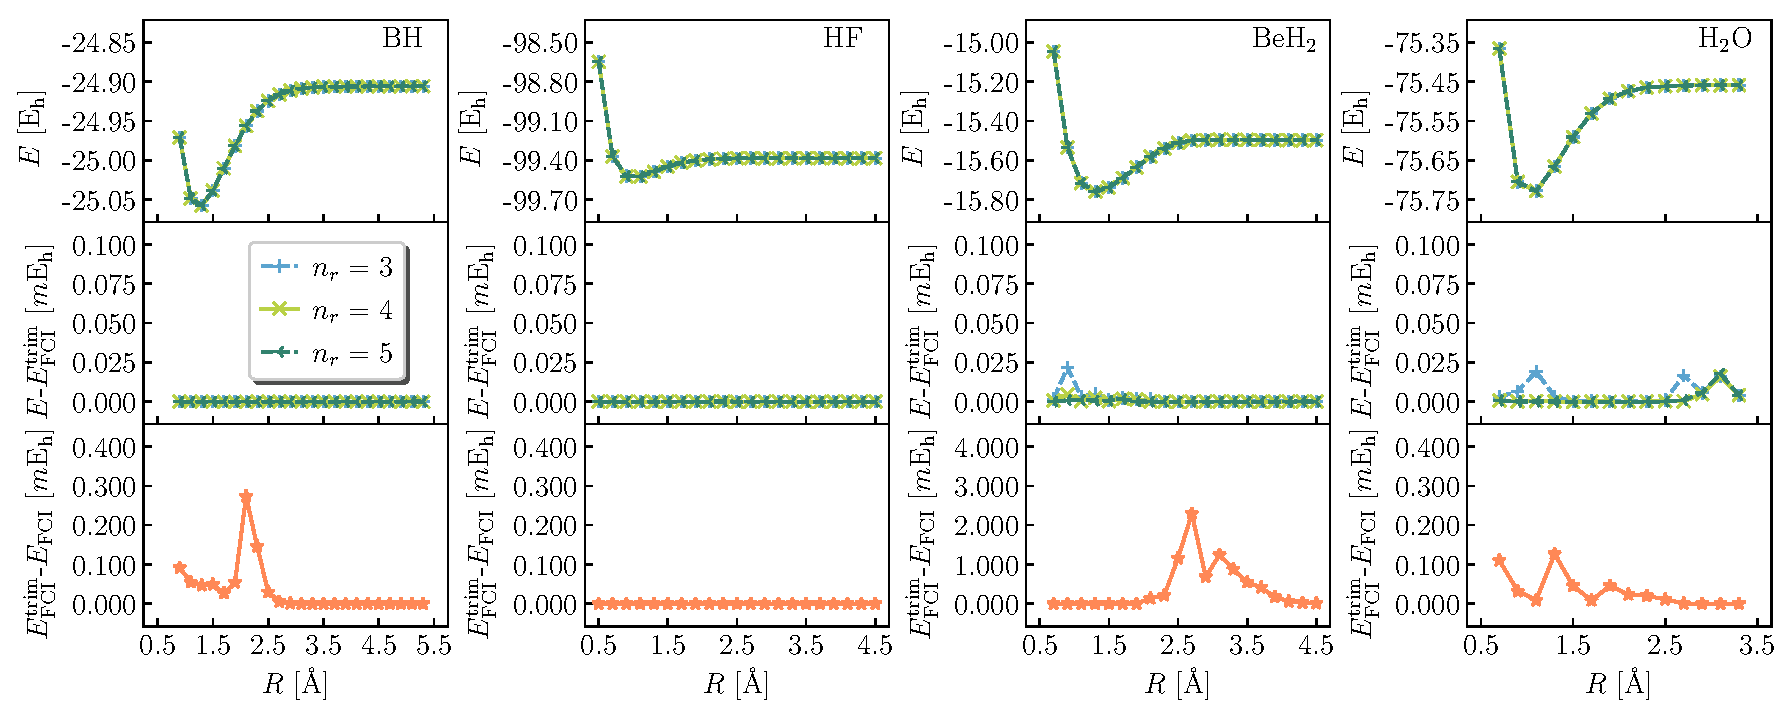
\includegraphics[width=0.9\textwidth]{../figures/first_quantization_trim/first_quantization_trim.eps}
\caption{Total energy, deviation between computed and exact total energy using a first-quantization encoding and a trimming procedure for qubit reduction,
and energy error from the trimming procedure (top to bottom) for the BH, HF, BeH$_2$ and H$_2$O molecules at STO-6G level (left to right) 
using the cascade Ansatz.}
\label{figure:first_trim}
\end{figure*} 

\begin{figure*}[t!]
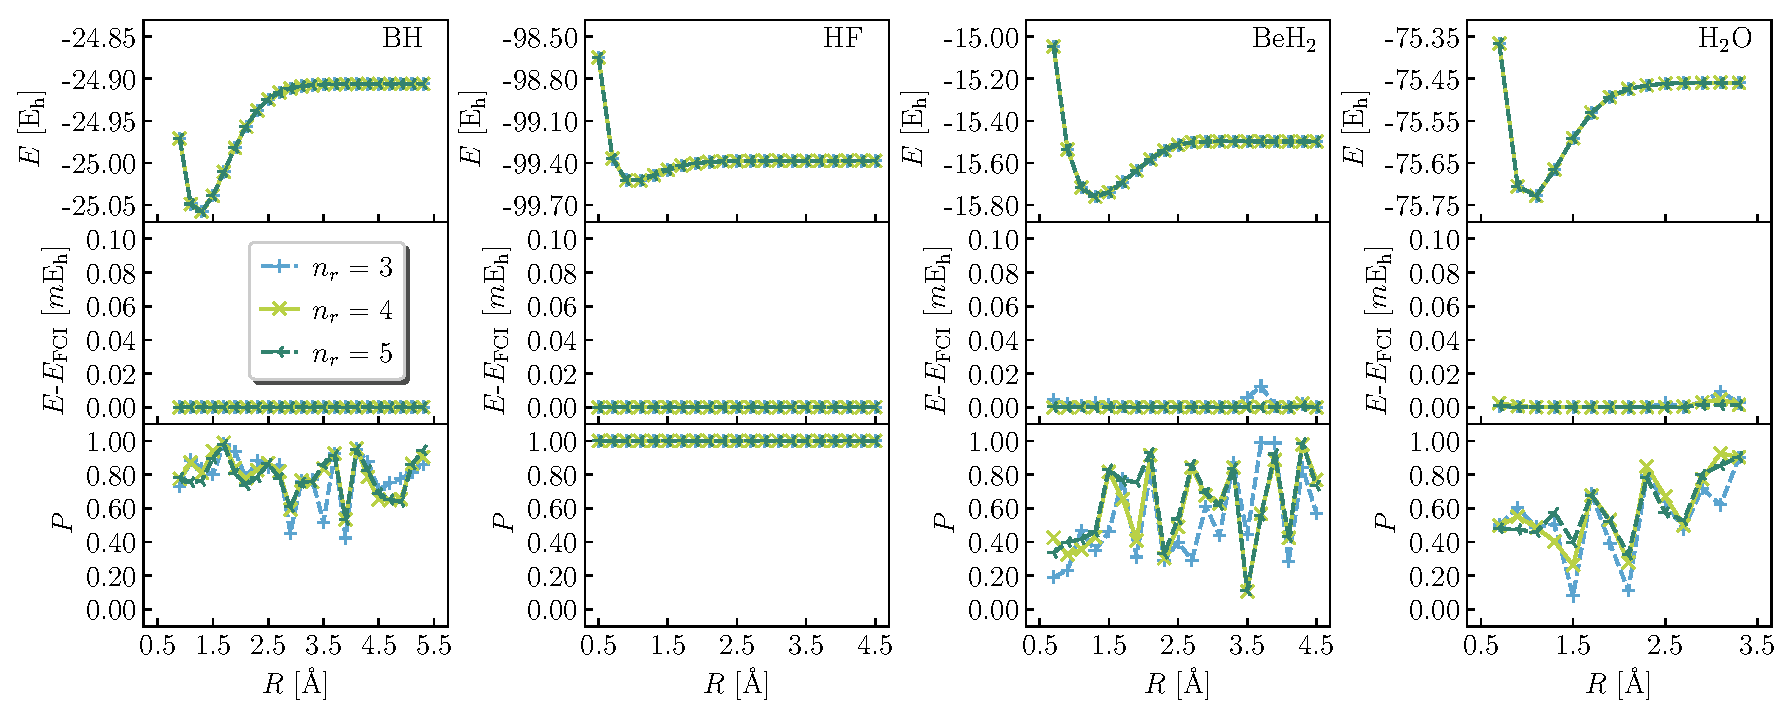
\includegraphics[width=0.9\textwidth]{../figures/first_quantization_pad_vap_cascade/first_quantization_pad_vap_cascade.eps}
\caption{Total energy, deviation between computed and exact energy, and squared-norm of the unphysical component of the wavefunction
(top to bottom) for the BH, HF, BeH$_2$ and H$_2$O molecules at STO-6G level (left to right) 
using a first-quantization encoding with padding and a cascade Ansatz optimized with the variation-after-projection scheme.}
\label{figure:first_pad_vap_cascade}
\end{figure*} 

\begin{figure*}[t!]
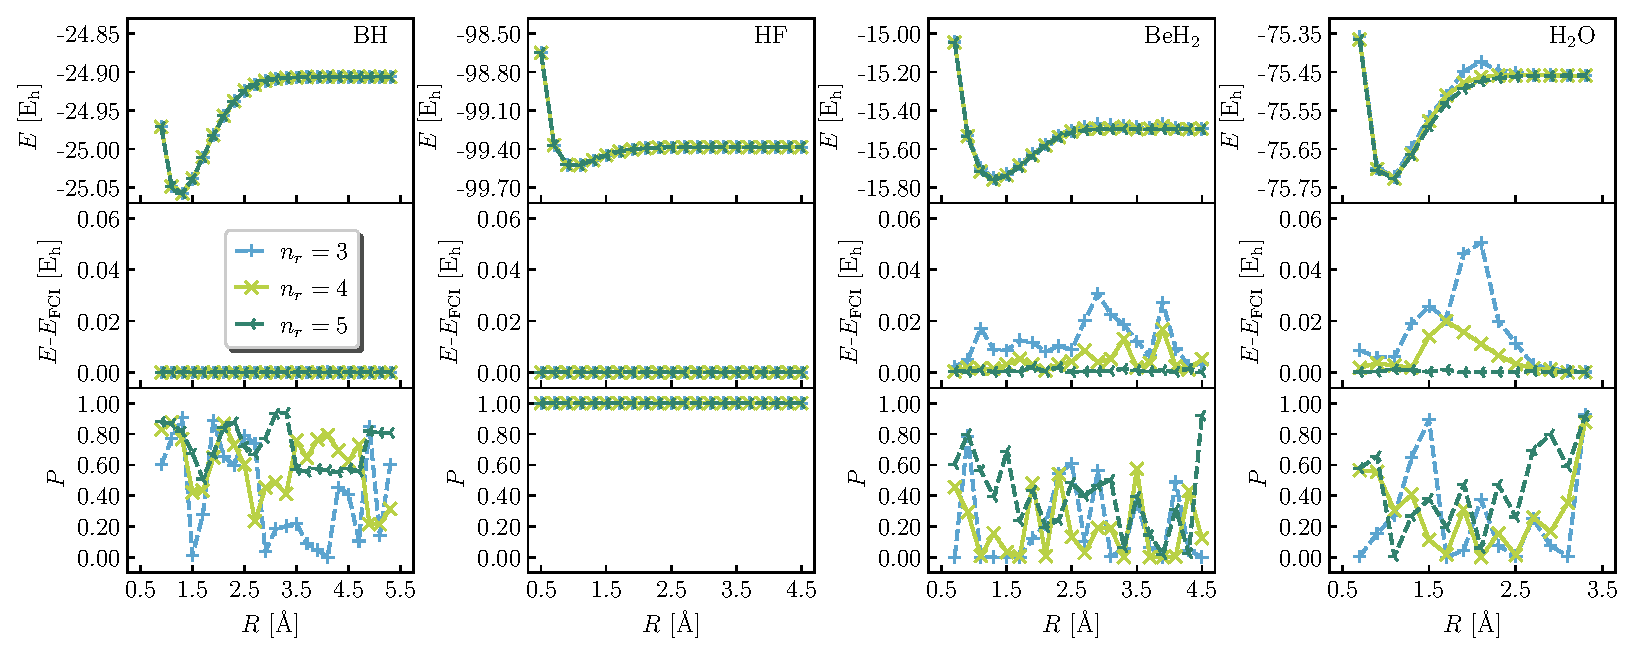
\includegraphics[width=0.9\textwidth]{../figures/first_quantization_pad_vap_ry_linear/first_quantization_pad_vap_ry_linear.eps}
\caption{Total energy, deviation between computed and exact energy, and squared-norm of the unphysical component of the wavefunction
(top to bottom) for the BH, HF, BeH$_2$ and H$_2$O molecules at STO-6G level (left to right) 
using a first-quantization encoding with padding and an R$_y$ Ansatz with linear connectivity optimized with the variation-after-projection scheme.}
\label{figure:first_pad_vap_ry}
\end{figure*} 

\section{Conclusions and outlooks}
\label{sec:conclusions}

\section*{Acknowledgments}


\appendix

\section{Closed-shell q-UCCSD}
\label{sec:cc_trotter}

\begin{figure*}[t!]
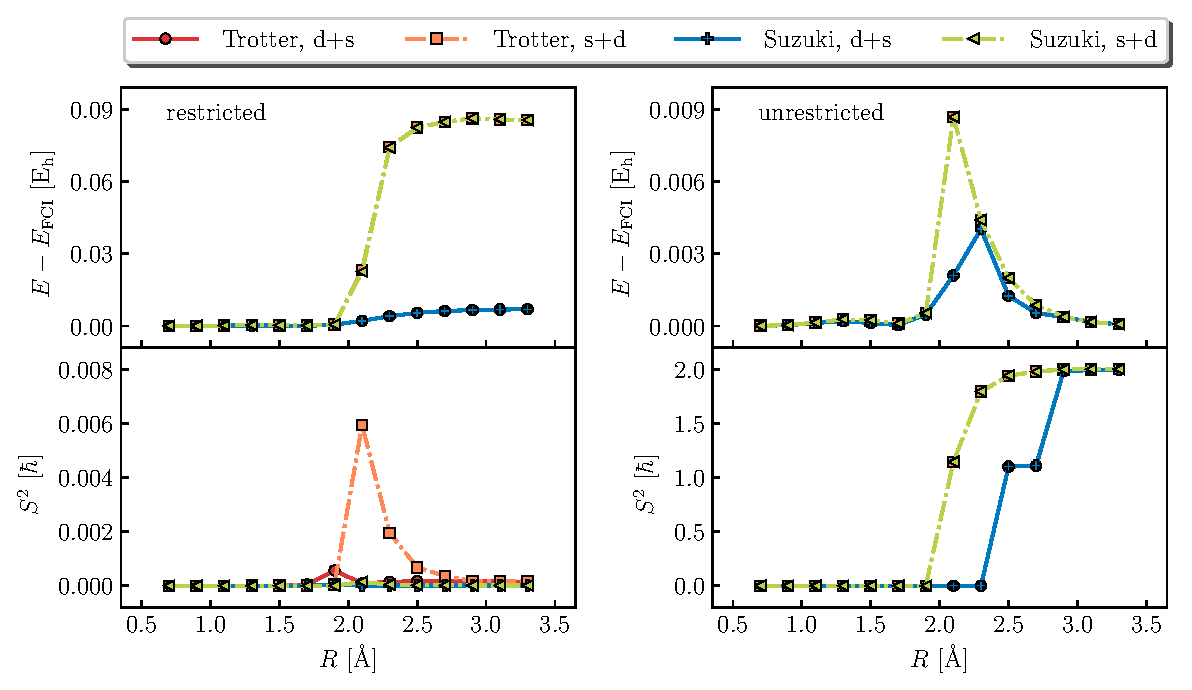
\includegraphics[width=0.7\textwidth]{../figures/qUCCSD_flavors/quccsd_reps_1.eps}
\caption{Deviation between computed and exact energy (top) and total spin (bottom), for the restricted closed-shell (left) and unrestricted (right) qUCCSD Ans\"{a}tze with $n_r=1$ repetitions, for the H$_2$O molecule at STO-6G level, using Trotter and Suzuki approximations (warm, cold colors) and with singles followed by doubles and doubles followed by singles (light, dark colors).}
\label{figure:quccsd_reps_1}
\end{figure*} 

\begin{figure*}[t!]
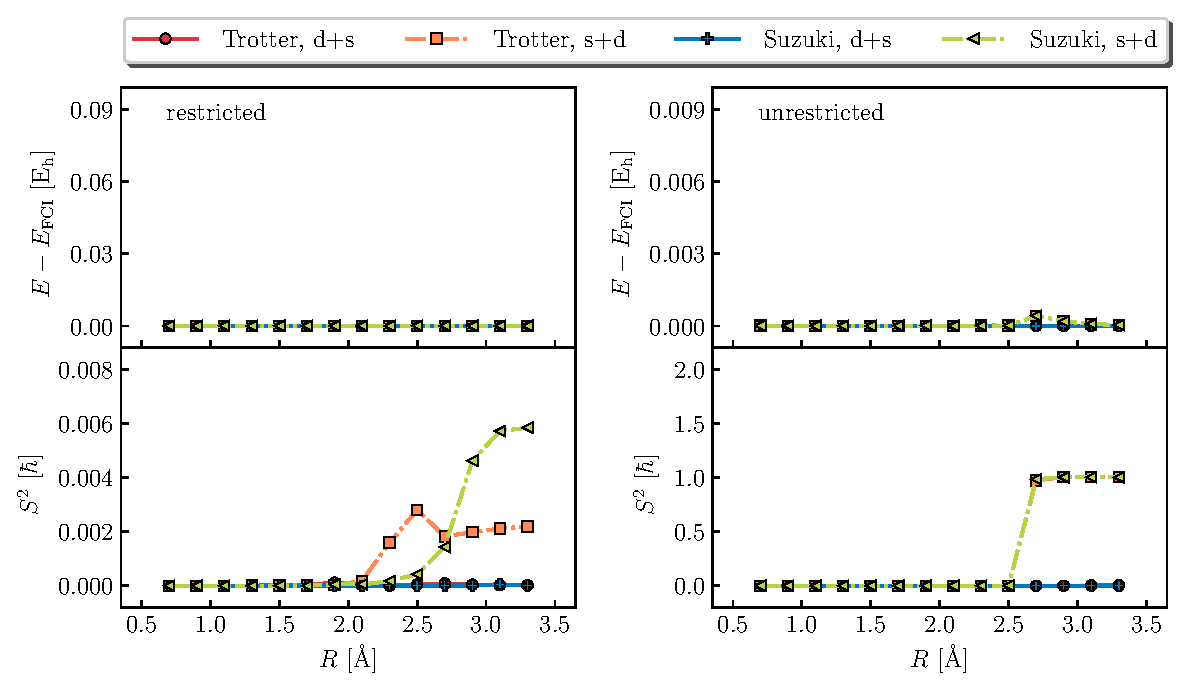
\includegraphics[width=0.7\textwidth]{../figures/qUCCSD_flavors/quccsd_reps_2.eps}
\caption{Deviation between computed and exact energy (top) and total spin (bottom), for the restricted closed-shell (left) and unrestricted (right) qUCCSD Ans\"{a}tze with $n_r=2$ repetitions, for the H$_2$O molecule at STO-6G level, using Trotter and Suzuki approximations (warm, cold colors) and with singles followed by doubles and doubles followed by singles (light, dark colors).}
\label{figure:quccsd_reps_2}
\end{figure*} 

\section{First quantization encoding}
\label{sec:first}

\section{Projection after variation}
\label{sec:pav}

\begin{figure}[t!]
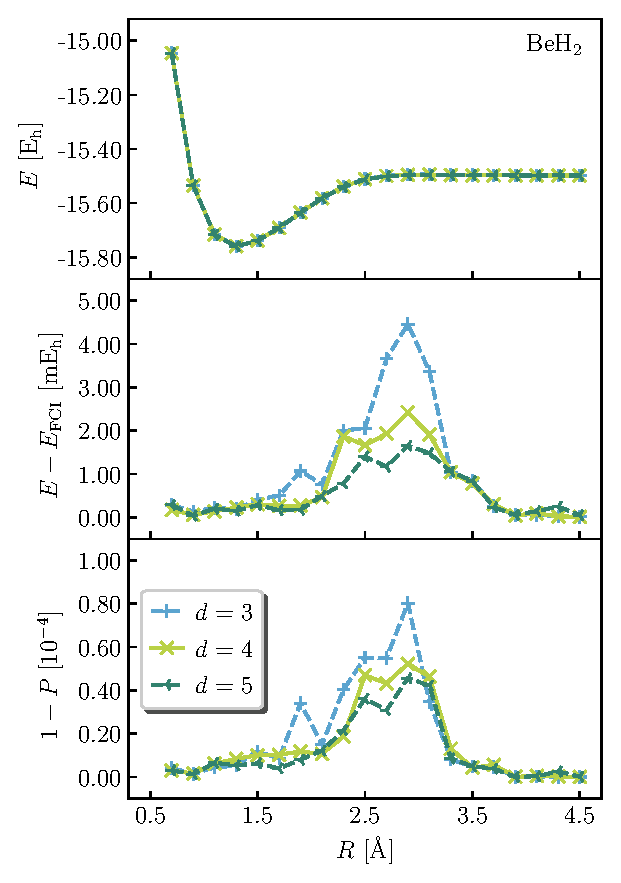
\includegraphics[width=0.4\textwidth]{../figures/first_quantization_pad_pav/first_quantization_pad_pav.eps}
\caption{Total energy, deviation between computed and exact energy, and squared-norm of the unphysical component of the wavefunction
(top to bottom) for the BeH$_2$ molecule at STO-6G level, 
using a first-quantization encoding with padding and a cascade Ansatz optimized with the projection-after-variation scheme.}
\label{figure:pad_pav}
\end{figure} 

\section{Classical preprocessing}
\label{sec:classical}

\begin{figure*}[t!]
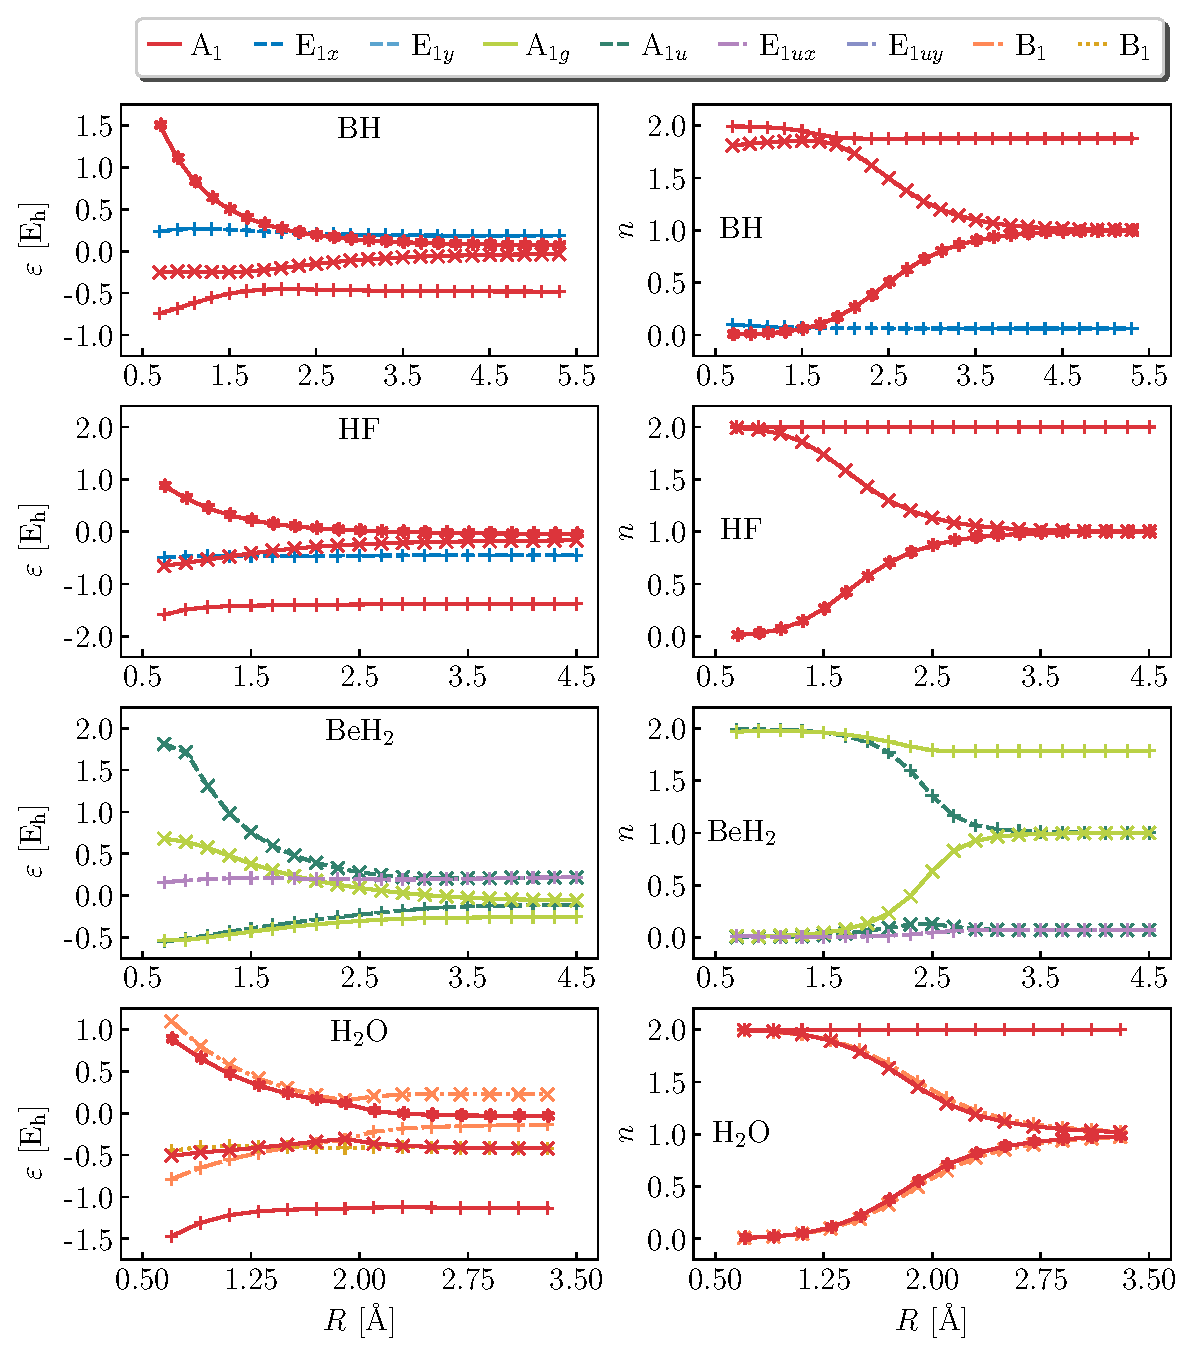
\includegraphics[width=0.6\textwidth]{../figures/scf_fci/scf_fci.eps}
\caption{Eigenvalues of the Fock operator in Hartree units (left, $\varepsilon$) and occupation numbers of the exact ground-state one-body density matrix (right, $n$) 
for BH, HF, BeH$_2$ and H$_2$O (top to bottom). 
Colors denote irreducible representations of the molecular point-group symmetry;
plus, cross, and asterisk markers denote orbitals in ascending order of energy within a specific irreducible representation;
the energy and occupation number of the core 1s orbital are omitted.}
\label{figure:scf}
\end{figure*}

\bibliographystyle{apsrev4-2}
\bibliography{main}

\end{document}
